%% Supplementary Information — build: latexmk -pdf supplementary.tex
\documentclass[12pt]{article}
\usepackage{graphicx}
\usepackage{booktabs}
\usepackage{amsmath}
\usepackage[margin=2.5cm]{geometry}
\usepackage[hidelinks]{hyperref}
\graphicspath{{figures/}}

\renewcommand{\thetable}{S\arabic{table}}
\renewcommand{\thefigure}{S\arabic{figure}}
\renewcommand{\thesection}{Text S\arabic{section}}

\title{Supplementary Information\\
Interpolation versus generalization in machine learning prediction of
micropollutant adsorption on layered double hydroxides}
\author{[AUTHORS]}
\date{}

\begin{document}
\maketitle

\section{Data cleaning rules}
All rules are implemented in \texttt{ldh\_pipeline.load\_data} and applied
identically in every notebook. (1) Column names are stripped of
surrounding whitespace. (2) Categorical labels are normalized by
lowercasing, collapsing internal whitespace and hyphen spacing, and
stripping trailing punctuation, after which known synonyms are merged
(e.g., \emph{co-precipitation or aging}, \emph{co- precipitation}
$\rightarrow$ \emph{Co-precipitation}; \emph{reconstruction or memory
effect} $\rightarrow$ \emph{Reconstruction}). (3) The removal ratio is
converted to percent units by a range-aware rule: if the column maximum
is $\le 1.5$ the values are multiplied by 100; an assertion then checks
that all values lie in $[0, 100]$, which makes the conversion idempotent
under re-execution. (4) Records identical in every descriptor are
reduced to their first occurrence (83 records removed). (5) Missing
numeric values are imputed inside each model pipeline by a five-neighbor
KNN imputer computed in z-score space and mapped back to physical units;
columns with no observed value in a training fold fall back to the fold
mean. The source-study identifier is retained for grouping only and
never enters the feature matrix.

\section{Hyperparameter search spaces and selected values}

Tree-ensemble hyperparameters were selected by Optuna (TPE sampler, 30
trials, seeded) on cross-validation folds of the training data of the
reference split; grid searches used the same folds. Selected values are
read directly from the saved model pipelines
(\texttt{Model/interp\_row\_42/saved\_models.joblib}).

\begin{table}[h]
\centering
\caption{Hyperparameter search spaces and selected values}
\begin{tabular}{lll}
\toprule
Model & Search space & Selected \\
\midrule
HistGB & max\_iter 100--600; lr $10^{-4}$--1 (log); depth 3--15; leaf 3--9 &
  max\_iter 484; lr 0.089; depth 14; leaf 8 \\
XGBoost & n\_estimators 100--600; lr $10^{-4}$--1 (log); depth 3--15;
  child weight 3--9 & 495 trees; lr 0.114; depth 13; child weight 7 \\
RF & n\_estimators 100--600; depth 3--15; leaf 3--9 &
  347 trees; depth 13; leaf 3 \\
Cubist & committees 1--9; neighbors none, 1--8 & committees 9; neighbors 1 \\
KNN & $k$ 1--9 & $k = 1$ \\
ANN & fixed: 1 hidden layer, 32 ReLU units, Adam, 2000 iterations & --- \\
LR & no hyperparameters & --- \\
\bottomrule
\end{tabular}
\end{table}

\section{Per-model results under both tasks}

\begin{table}[h]
\centering
\caption{Leave-one-study-out per-study MAE distribution (RR\%),
59 studies, fixed hyperparameters}
\begin{tabular}{lccc}
\toprule
Model & Median & Q25 & Q75 \\
\midrule
Cubist & 14.1 & 4.7 & 22.2 \\
KNN    & 16.0 & 6.5 & 30.3 \\
HistGB & 16.4 & 4.7 & 25.8 \\
RF     & 16.8 & 6.1 & 25.9 \\
ANN    & 18.1 & 11.5 & 38.6 \\
XGB    & 18.3 & 3.8 & 25.4 \\
LR     & 28.4 & 18.4 & 34.8 \\
\midrule
Global-mean baseline & 24.2 & -- & -- \\
Per-pollutant-mean baseline & 25.1 & -- & -- \\
\bottomrule
\end{tabular}
\end{table}

\begin{table}[h]
\centering
\caption{Wall-clock training and prediction time on the reference split
(seconds; single measurement, indicative only)}
\begin{tabular}{lcc}
\toprule
Model & Fit & Predict \\
\midrule
KNN & 0.05 & 0.04 \\
LR & 0.14 & 0.05 \\
Cubist & 0.22 & 0.04 \\
RF & 0.37 & 0.09 \\
ANN & 0.67 & 0.01 \\
HistGB & 0.86 & 0.08 \\
XGBoost & 10.1 & 0.03 \\
\bottomrule
\end{tabular}
\end{table}

\section{Extended statistical description}

\begin{table}[h]
\centering
\small
\caption{Extended descriptor statistics}
\begin{tabular}{lcccccc}
\toprule
Descriptor & Mean & SD & Median & Range & Skewness & Missing (\%) \\
\midrule
log $K_{\mathrm{ow}}$ & 0.83 & 2.34 & $-0.02$ & $-2.67$--4.51 & 0.5 & 0 \\
MW (g/mol) & 349.4 & 97.1 & 331.3 & 152.2--733.9 & 0.5 & 0 \\
$E$ & 2.04 & 0.75 & 1.81 & 0.70--3.60 & 0.8 & 0 \\
$S$ & 2.33 & 0.71 & 2.10 & 0.70--3.60 & 0.4 & 0 \\
$A$ & 0.83 & 0.38 & 0.70 & 0.31--1.65 & 0.8 & 0 \\
$B$ & 1.73 & 0.94 & 1.70 & 0.45--3.50 & 0.5 & 0 \\
$V$ & 2.41 & 0.76 & 2.30 & 1.13--6.35 & 2.0 & 0 \\
TPSA (\AA$^2$) & 101.7 & 55.1 & 76.2 & 37.3--194.0 & 0.6 & 0 \\
M(II)/M(III) & 3.02 & 1.21 & 3.00 & 0.50--8.00 & 1.9 & 0 \\
Avg.\ atomic weight (g/mol) & 42.8 & 16.2 & 48.1 & 24.8--73.7 & 0.1 & 0 \\
Avg.\ d-electrons & 3.77 & 3.69 & 4.25 & 0--8.89 & 0.1 & 0 \\
Avg.\ Pauling electronegativity & 1.59 & 0.17 & 1.59 & 1.30--1.89 & 0.4 & 0 \\
Hydrothermal temp.\ (\textcelsius) & 78.6 & 28.6 & 70 & 25--160 & 1.5 & 13.3 \\
Hydrothermal time (h) & 22.9 & 4.6 & 24 & 12--40 & $-0.1$ & 13.3 \\
Calcination temp.\ (\textcelsius) & 414 & 73 & 400 & 200--550 & $-0.3$ & 66.0 \\
Calcination time (h) & 4.7 & 3.0 & 4 & 1--12 & 1.3 & 66.0 \\
$d_{003}$ (nm) & 0.78 & 0.11 & 0.77 & 0.25--1.13 & $-0.8$ & 2.5 \\
BET (m$^2$/g) & 85.7 & 57.6 & 82.0 & 0.4--225.7 & 0.5 & 7.9 \\
PV (cm$^3$/g) & 0.24 & 0.33 & 0.10 & 0--1.46 & 2.2 & 25.3 \\
APD (nm) & 12.2 & 12.0 & 8.4 & 0.2--64.2 & 1.6 & 13.9 \\
pH$_{\mathrm{pzc}}$ & 8.02 & 1.56 & 7.50 & 5.50--11.56 & 0.7 & 24.6 \\
pH & 6.50 & 2.19 & 6.70 & 2.0--12.0 & 0.3 & 0 \\
Temperature (\textcelsius) & 25.3 & 2.9 & 25 & 10--55 & 2.6 & 0 \\
Contact time (h) & 9.9 & 33.3 & 1.5 & 0.02--192 & 4.9 & 0 \\
Dose (g/L) & 2.57 & 6.38 & 0.90 & 0.01--50 & 6.0 & 0 \\
$C_i$ (mg/L) & 94.4 & 188.9 & 40 & 1--1688 & 5.0 & 0 \\
\bottomrule
\end{tabular}
\end{table}

\begin{table}[h]
\centering
\small
\caption{Composition of the compilation by pollutant, metal, and
synthesis route (records / source studies)}
\begin{tabular}{lcc@{\qquad}lcc}
\toprule
Level & Rec. & St. & Level & Rec. & St. \\
\midrule
\multicolumn{3}{l}{\emph{Micropollutant}} & \multicolumn{3}{l}{\emph{Metal(II)}} \\
Diclofenac & 304 & 3 & Mg & 633 & 15 \\
Tetracycline & 208 & 8 & Zn & 312 & 31 \\
Ciprofloxacin & 181 & 32 & Ni & 162 & 7 \\
Doxycycline & 106 & 3 & Cu & 92 & 3 \\
Levofloxacin & 102 & 3 & ZnCo & 58 & 2 \\
Amoxicillin & 94 & 3 & Ca & 34 & 1 \\
Norfloxacin & 90 & 1 & NiAl & 28 & 1 \\
Metronidazole & 81 & 1 & CoZn & 23 & 1 \\
Methylparaben & 56 & 1 & \multicolumn{3}{l}{\emph{Metal(III)}} \\
Ibuprofen & 39 & 1 & Al & 819 & 47 \\
Moxifloxacin & 25 & 1 & Fe & 311 & 12 \\
Delafloxacin & 23 & 1 & TiAl & 153 & 1 \\
Erythromycin & 22 & 1 & Ce & 31 & 1 \\
Oxytetracycline & 11 & 1 & Ti & 28 & 1 \\
\midrule
\multicolumn{6}{l}{\emph{Synthesis route}} \\
Co-precipitation & 1171 & 54 & Urea hydrolysis & 132 & 3 \\
Hydrothermal & 28 & 1 & Reconstruction & 11 & 1 \\
\bottomrule
\end{tabular}
\end{table}

\begin{table}[h]
\centering
\caption{Variance inflation factors of the numeric descriptors (six
largest; 22 of 26 exceed 10)}
\begin{tabular}{lc}
\toprule
Descriptor & VIF \\
\midrule
Hydrothermal temperature & $2.5 \times 10^{6}$ \\
Hydrothermal time & $1.6 \times 10^{6}$ \\
$d_{003}$ & $1.1 \times 10^{6}$ \\
$A$ & $7.8 \times 10^{5}$ \\
Calcination temperature & $4.2 \times 10^{5}$ \\
PV & $3.4 \times 10^{5}$ \\
\bottomrule
\end{tabular}
\end{table}

\begin{table}[h]
\centering
\caption{Share of total mean $|$SHAP$|$ attribution by descriptor group
(HistGB, hold-out test)}
\begin{tabular}{lc}
\toprule
Descriptor group & Share (\%) \\
\midrule
Operating conditions & 54.2 \\
Material texture & 17.8 \\
Composition and synthesis & 14.4 \\
Micropollutant descriptors & 13.5 \\
\bottomrule
\end{tabular}
\end{table}

\begin{table}[h]
\centering
\caption{Feature-set comparison for XGBoost and Cubist (interpolation
mean $\pm$ SD over 20 splits)}
\begin{tabular}{llcc}
\toprule
Feature set & Model & Interp.\ $R^2$ & Interp.\ MAE \\
\midrule
Full (30) & XGBoost & $0.84 \pm 0.03$ & $6.3 \pm 0.6$ \\
Full (30) & Cubist & $0.79 \pm 0.03$ & $8.0 \pm 0.6$ \\
Correlation-screened (21) & XGBoost & $0.84 \pm 0.03$ & $6.4 \pm 0.6$ \\
Correlation-screened (21) & Cubist & $0.79 \pm 0.04$ & $8.2 \pm 0.6$ \\
Top-10 permutation & XGBoost & $0.84 \pm 0.03$ & $6.4 \pm 0.6$ \\
Top-10 permutation & Cubist & $0.79 \pm 0.03$ & $8.1 \pm 0.5$ \\
\bottomrule
\end{tabular}
\end{table}

\section{Additional figures}

\begin{figure}[h]
\centering
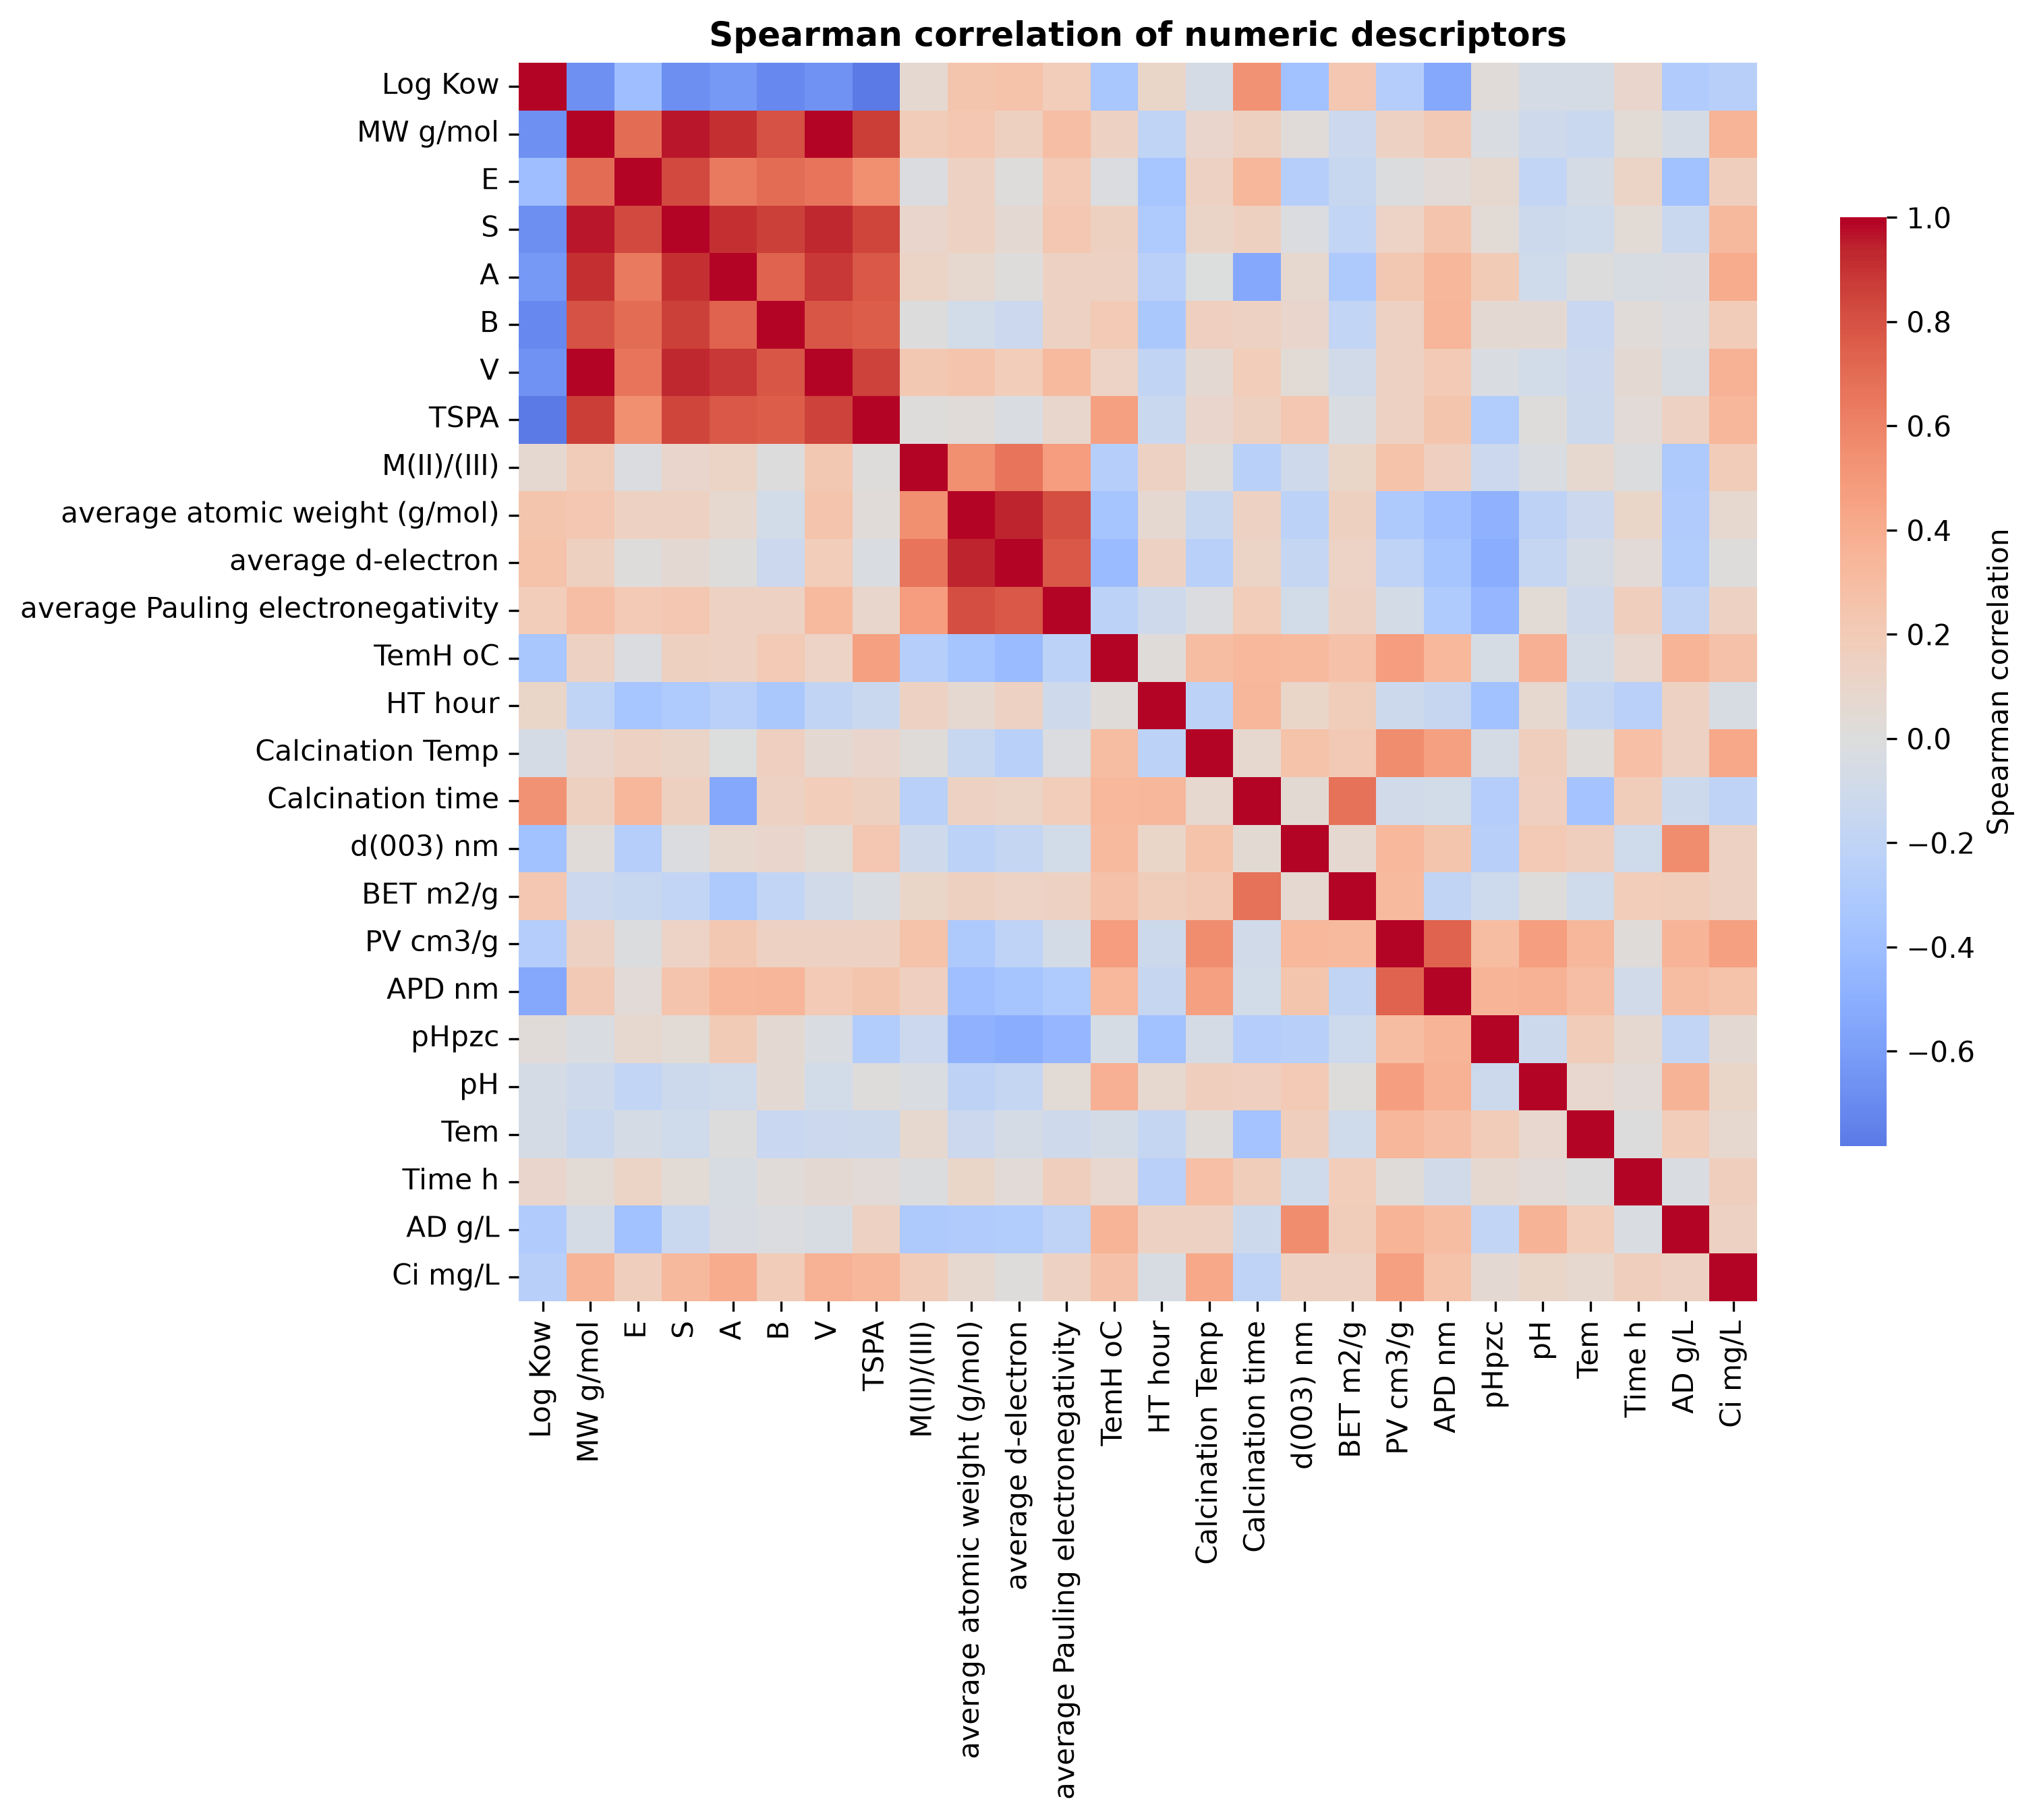
\includegraphics[width=.85\linewidth]{fig_corr_heatmap}
\caption{Spearman correlation of the numeric descriptors}
\end{figure}

\begin{figure}[h]
\centering
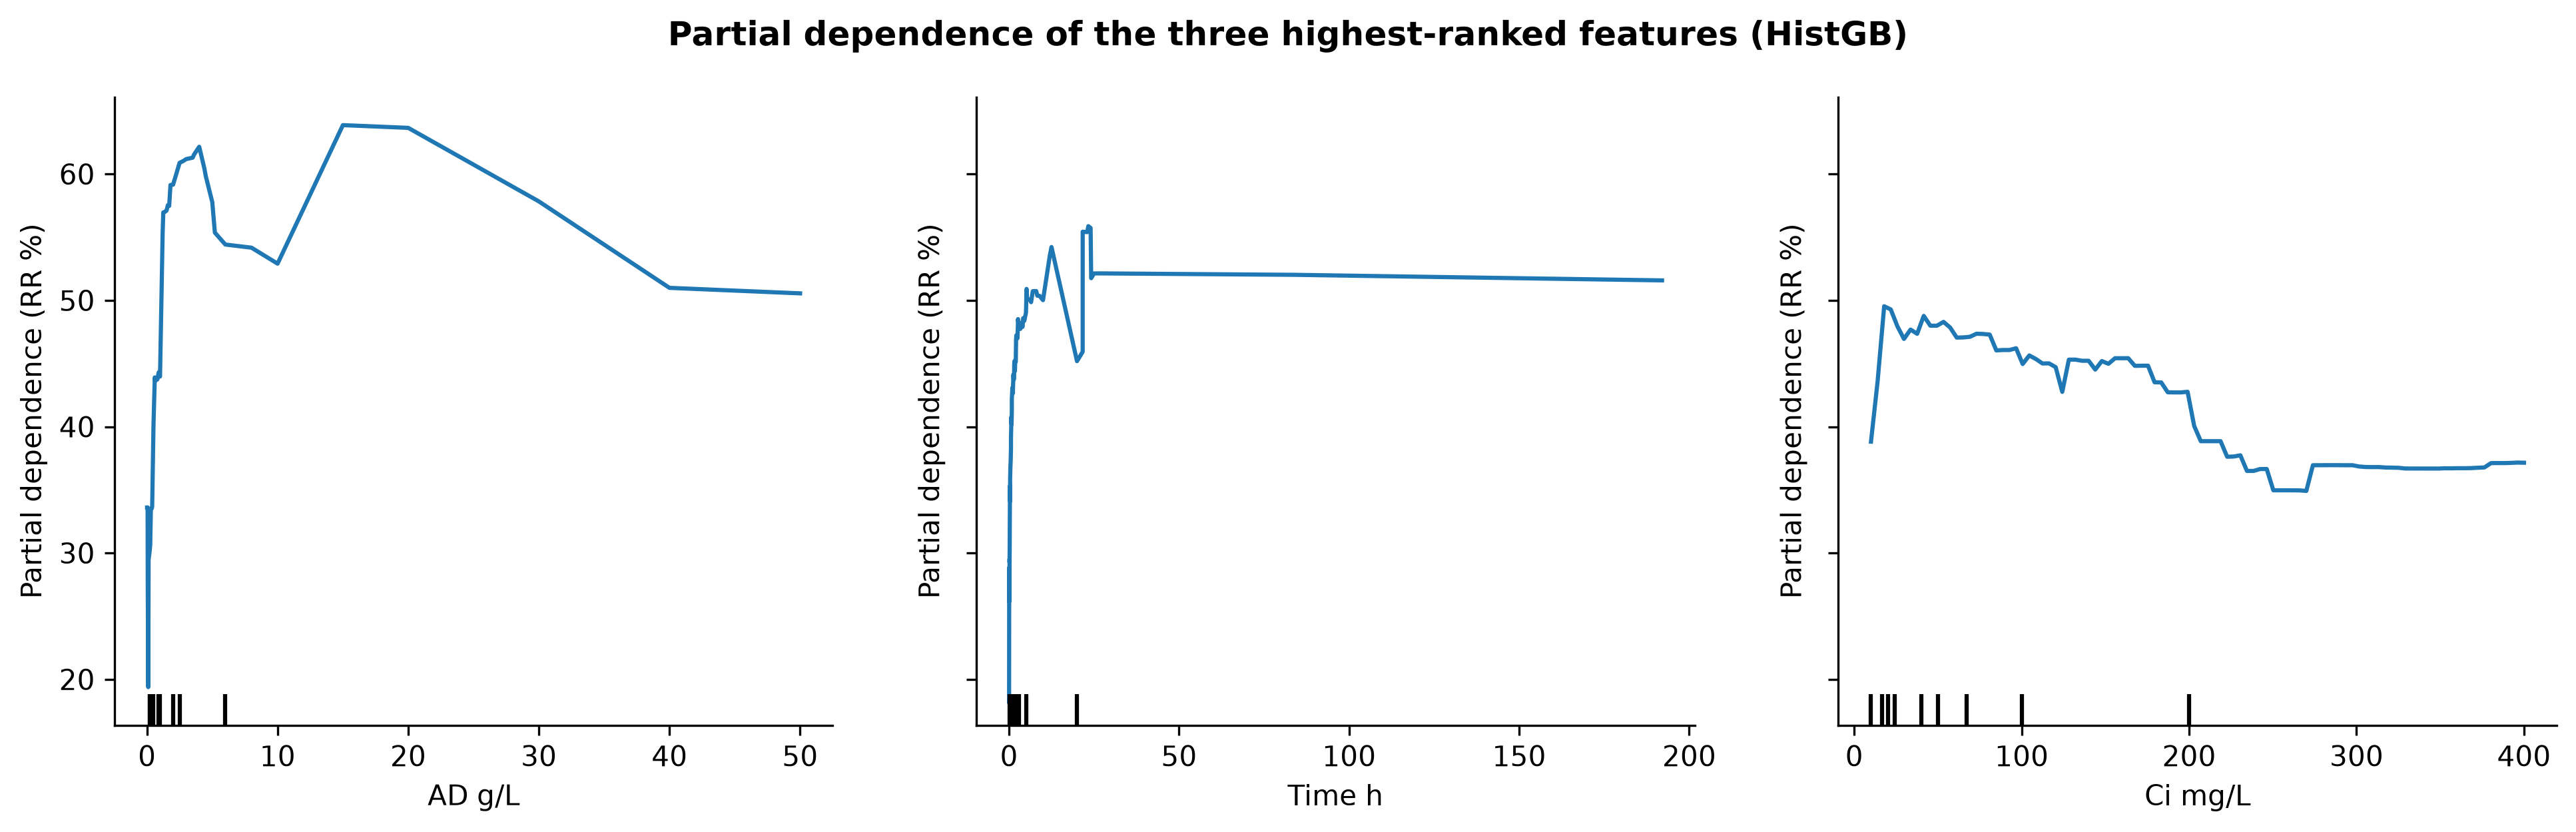
\includegraphics[width=.95\linewidth]{fig_pdp}
\caption{Partial dependence of the three highest-ranked features (HistGB)}
\end{figure}

\begin{figure}[h]
\centering
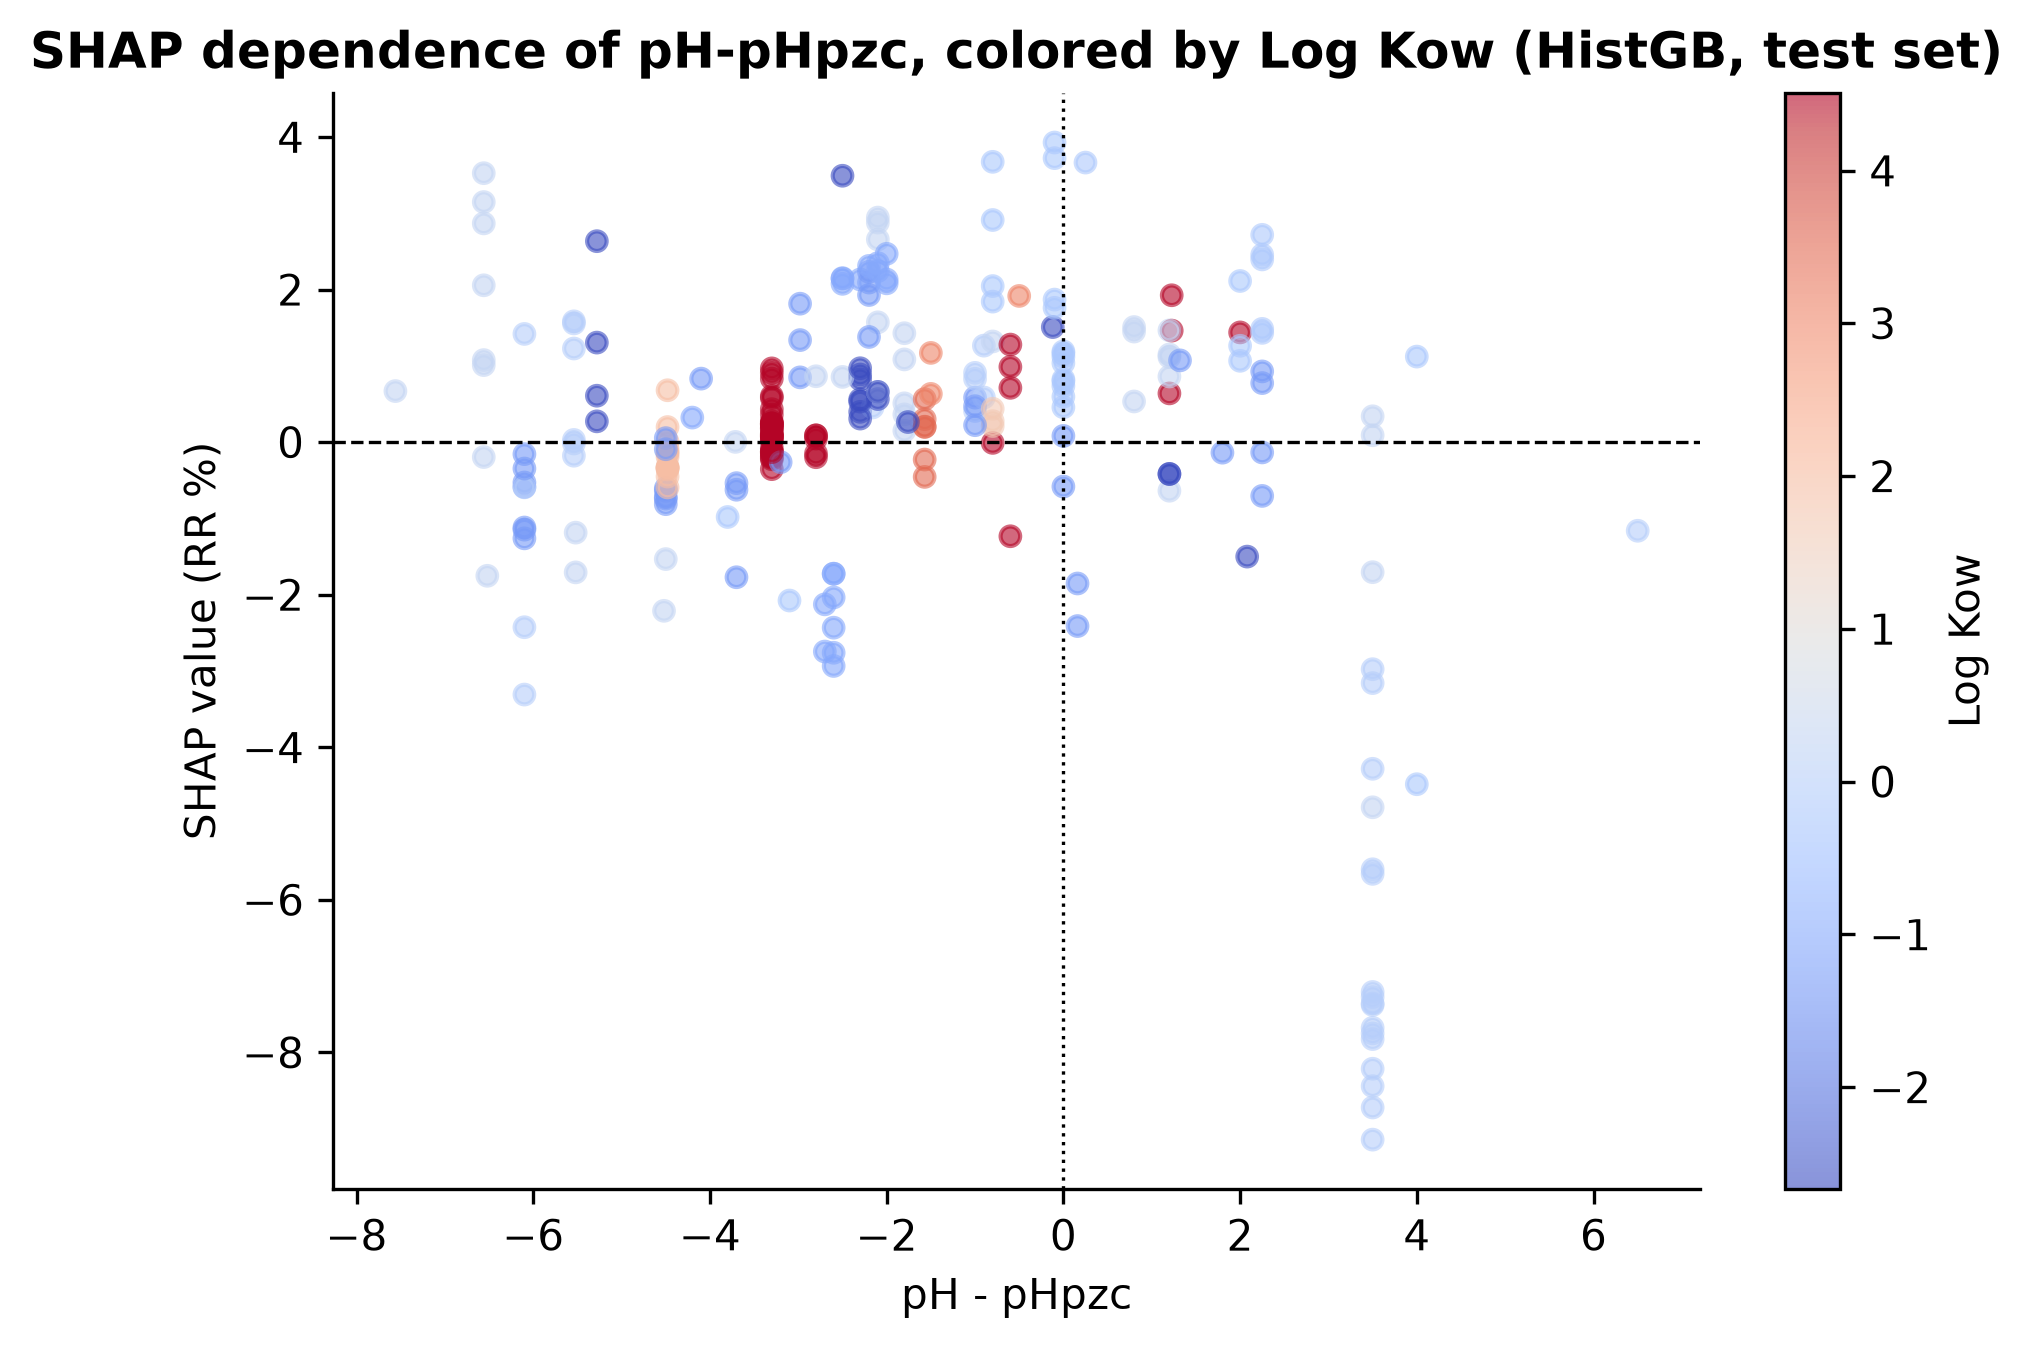
\includegraphics[width=.7\linewidth]{fig_shap_interaction}
\caption{SHAP dependence of pH$-$pH$_{\mathrm{pzc}}$ colored by log
$K_{\mathrm{ow}}$ (HistGB with engineered features, hold-out test set)}
\end{figure}

\begin{figure}[h]
\centering
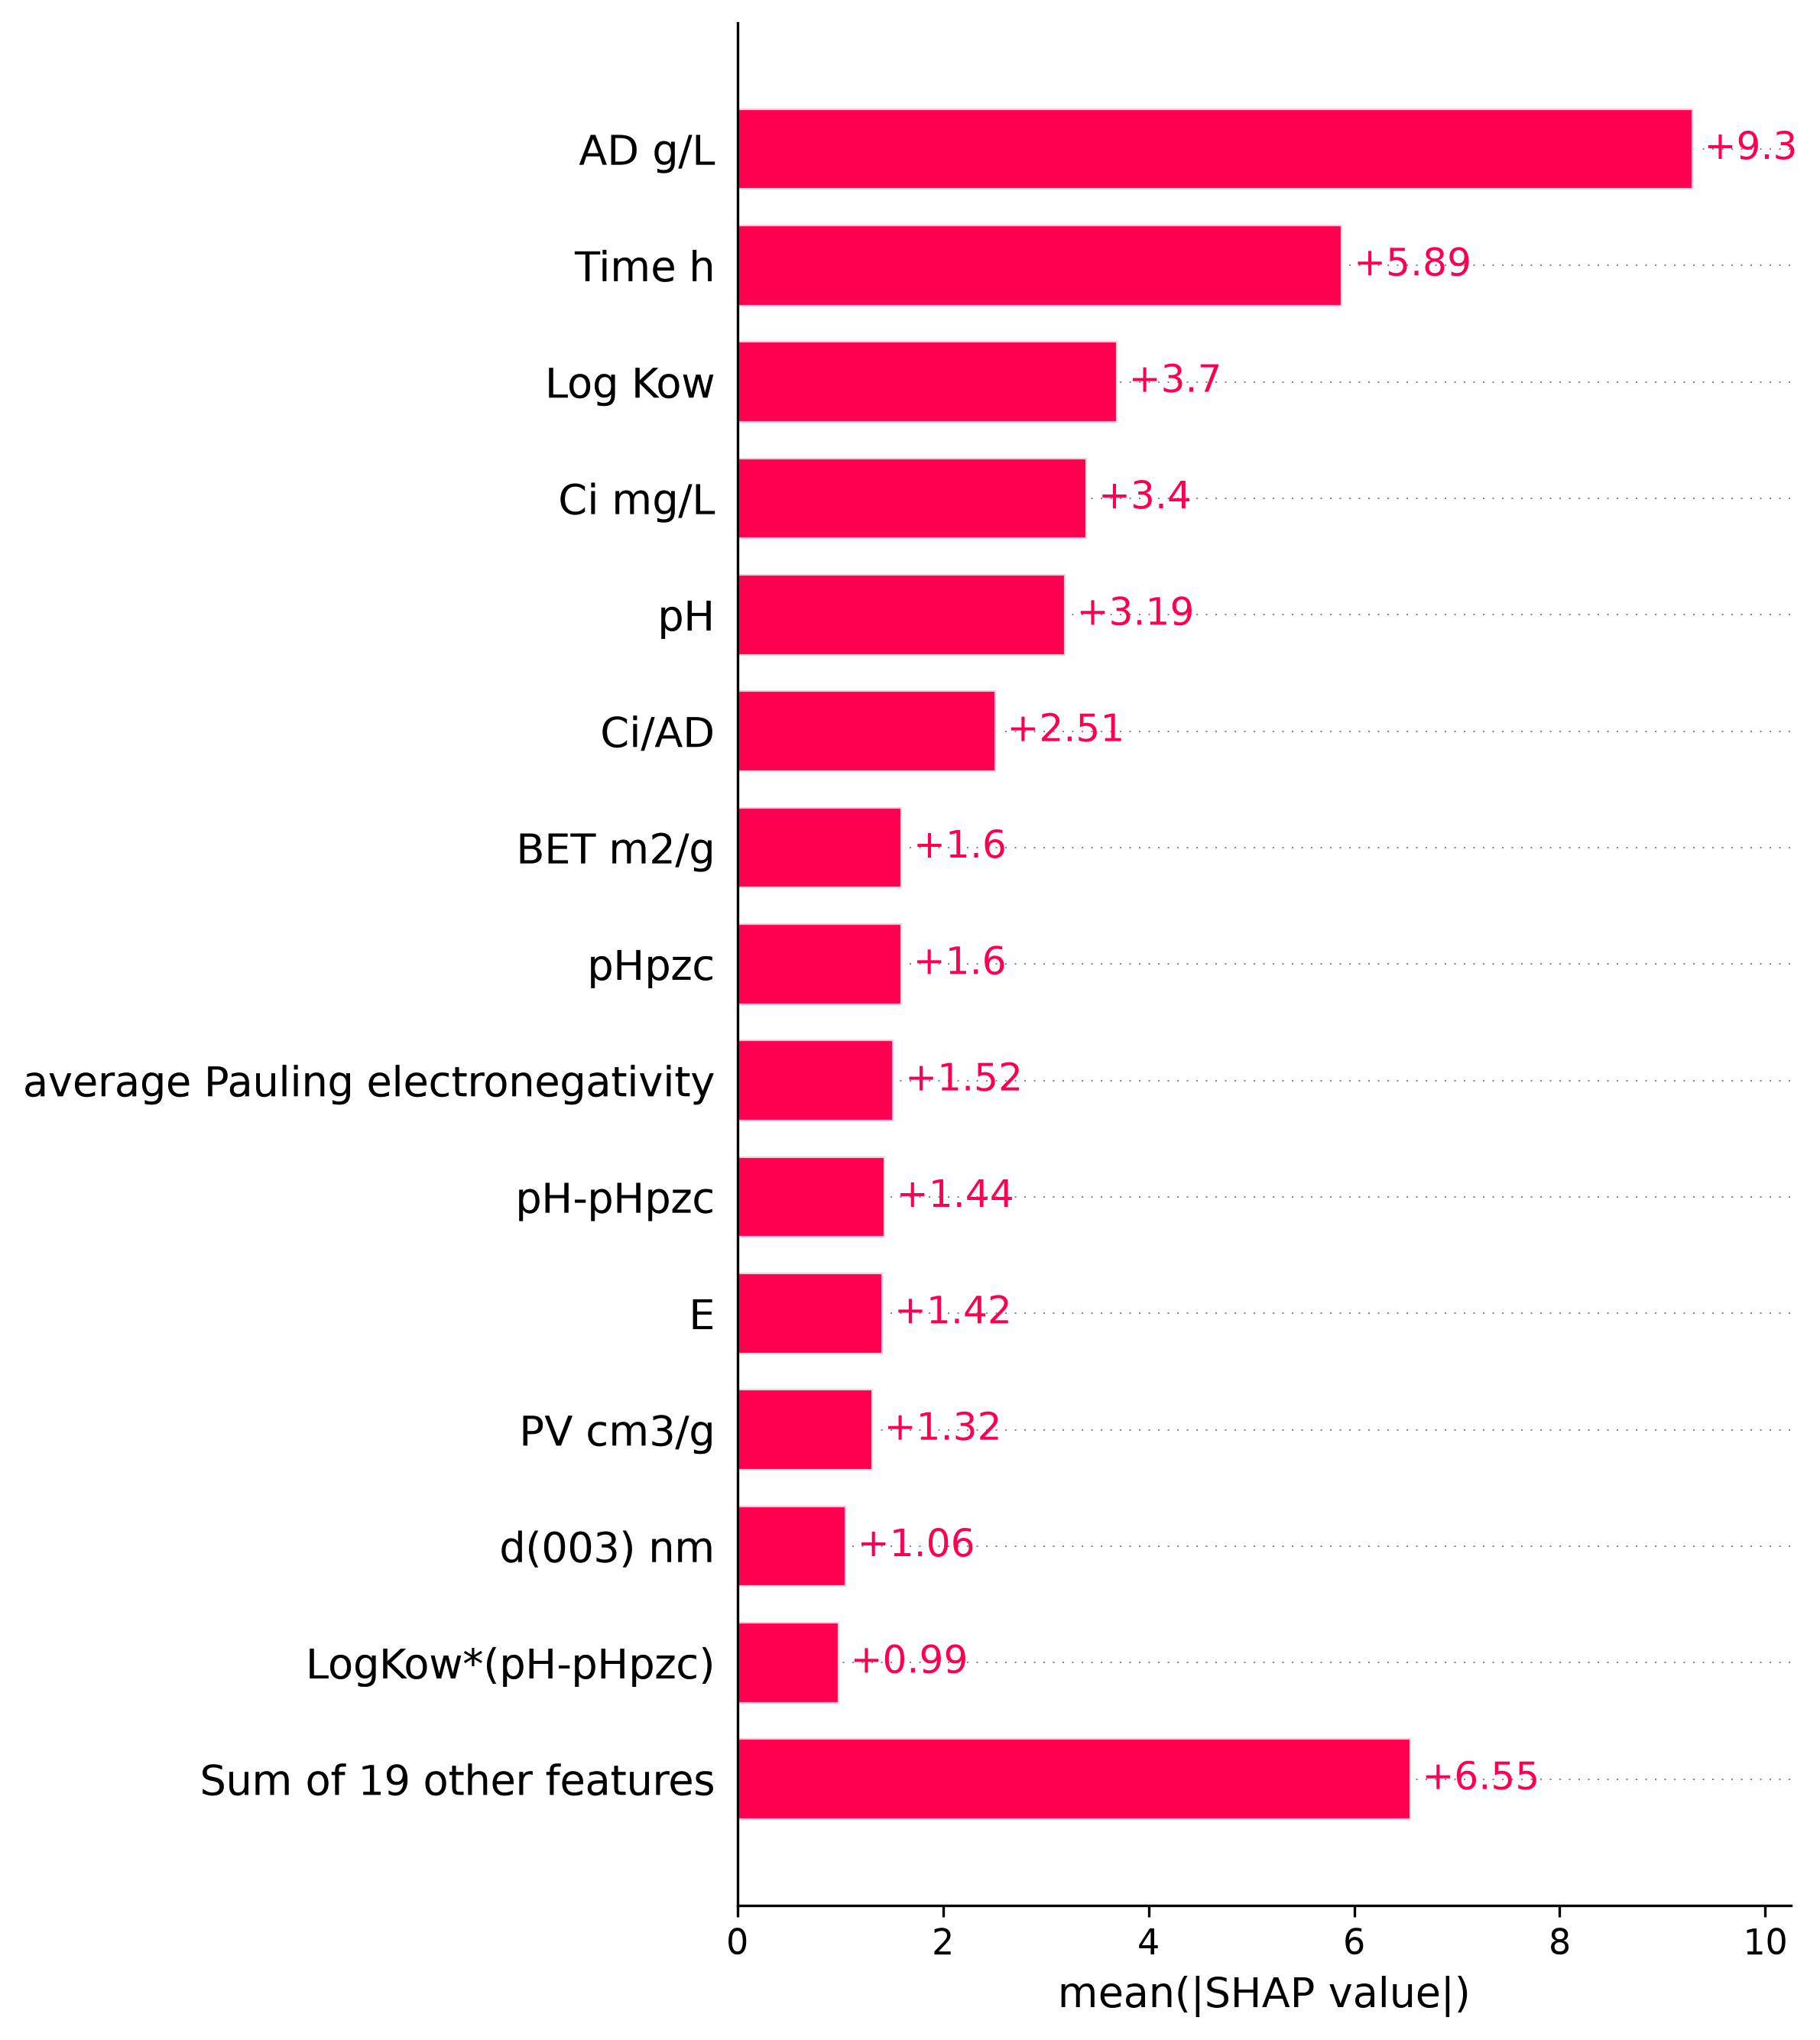
\includegraphics[width=.8\linewidth]{fig_shap_bar_eng}
\caption{Global SHAP importance, HistGB with engineered features}
\end{figure}

\end{document}
